\documentclass[11pt]{article}

\usepackage[a4paper,margin=1in]{geometry}
\usepackage[T1]{fontenc}
\usepackage[utf8]{inputenc}
\usepackage{lmodern}
\usepackage{microtype}
\usepackage{amsmath,amssymb,amsthm,mathtools}
\usepackage{booktabs}
\usepackage{graphicx}
\usepackage{float}
\usepackage{placeins}
\usepackage{enumitem}
\usepackage[numbers,sort&compress]{natbib}
\usepackage{xcolor}
\usepackage{xurl}
\usepackage[colorlinks=true,linkcolor=blue!55!black,citecolor=blue!55!black,urlcolor=blue!55!black]{hyperref}
\usepackage[nameinlink,noabbrev]{cleveref}

\setlength{\parindent}{1.4em}
\setlength{\parskip}{0.15em}
\setlist{itemsep=0.25em,topsep=0.35em}

\newtheorem{theorem}{Theorem}[section]
\newtheorem{proposition}[theorem]{Proposition}
\newtheorem{lemma}[theorem]{Lemma}
\newtheorem{corollary}[theorem]{Corollary}
\theoremstyle{definition}
\newtheorem{definition}[theorem]{Definition}
\theoremstyle{remark}
\newtheorem{remark}[theorem]{Remark}

\newcommand{\R}{\mathbb R}
\newcommand{\C}{\mathbb C}
\newcommand{\uc}{u_{\mathrm c}}
\newcommand{\Id}{\mathrm I}
\newcommand{\cK}{\mathcal K}
\newcommand{\cT}{\mathcal T}
\newcommand{\cR}{\mathcal R}
\newcommand{\cF}{\mathcal F}
\newcommand{\cH}{\mathcal H}
\newcommand{\spec}{\operatorname{spec}}
\newcommand{\spr}{\operatorname{spr}}

\title{\textbf{Complement Coupling in Time-Unfolded}\\
\textbf{Gaussian Returns at a Quadratic Band-Merging Map:}\\[0.35em]
\large Critical-Sibling Leakage, Floquet Replication, and a No-Go Theorem\\
for Naive Feshbach Identification}
\author{Liang Wang\\
\small School of Artificial Intelligence and Automation,\\[-0.2em]
\small Huazhong University of Science and Technology, Wuhan 430074, P.R. China\\
\small \texttt{wangliang.f@gmail.com}}
\date{July 2026}

\begin{document}

\maketitle

\begin{abstract}
At the first algebraic band-merging parameter of
$f_u(x)=1-u x^2$, a branch-isolated return of the exact Gaussian Markov
operator gives a roots-of-unity ring whose principal radius accurately
locates the observed small-noise bulk spectral edge.  The missing step is a
Feshbach theorem showing that the discarded complement only produces a
controlled Schur self-energy.  We prove that the most direct version of this
step cannot work.

The first obstruction is dynamical.  In the critical scaling
$\delta/\sigma\to d$, the endpoint Gaussian pulls back to the conditioned
Gaussian--quadratic profile $\Gamma_{d,t}$.  Its exact reflection symmetry
about the physical partition $b=u_{\mathrm c}^{-1/2}$ implies
\[
 \frac{\|\mathbf1_{x>b}\mathcal K_\sigma^2g_\sigma\|_{L^2(\mathrm{critical})}}
 {\|\mathbf1_{x<b}\mathcal K_\sigma^2g_\sigma\|_{L^2(\mathrm{critical})}}
 \longrightarrow1.
\]
Thus the omitted critical sibling is not a Gaussian tail.  The conclusion
persists under the Riccati time weights because both branches occur at the
same time slice.  Splitting the final window into left and right pieces gives
an exact operator identity
$R^{\rm both}=R^-+R^+$.

The second obstruction is algebraic.  If $T=\mathcal K_\sigma^2$ and the
full time-unfolded operator on $\mathcal H^k$ is
$(\mathfrak C_kv)_j=Tv_{j+1}$, then discrete Fourier transformation gives
\[
 \mathfrak C_k\simeq\bigoplus_{\ell=0}^{k-1}\omega_k^\ell T,
 \qquad
 \det(\Id-z\mathfrak C_k)=\det(\Id-z^kT^k).
\]
Hence every single physical eigenvalue of $T$ generates a complete
roots-of-unity ring in the time lift.  After the canonical bipartite lift,
one physical eigenvalue of $\mathcal K_\sigma$ generates $2k$ artificial
rotations.  A sector-free Feshbach completion of the local cyclic block can
therefore recover only this replicated spectrum; it cannot by itself prove
that the physical Markov operator has $2k$ distinct resonances.

We write the exact Schur self-energy for phase-dependent packet projections
and show separately that global Perron/parity deflation does not commute with
localization.  Seven-noise sparse computations support the analytic
obstruction.  At $\sigma=10^{-4}$, the right-sibling exit norm is $0.99738$
of the retained left mass and its return eigenvalue is $0.99476$ of the left
return.  Combining both branches changes the one-step radius from
$0.75646$ to $0.78982$; the unrestricted endpoint return is $0.78992$.
These are ordinary floating-point diagnostics.  The negative result does not
invalidate the deterministic pole or the observed cloud.  It replaces the
naive scalar Feshbach target by a branch-resolved, Floquet-sector effective
Hamiltonian in which peripheral extraction is built into the entrance and
exit maps.
\end{abstract}

\noindent\textbf{Keywords:} Gaussian transfer operator; Feshbach map;
Schur complement; Floquet decomposition; critical branch; spectral
deflation; non-normal spectrum; quadratic map.

\medskip
\noindent\textbf{MSC 2020:} 37E05; 37D25; 47A10; 47A55; 47B65; 60J05;
65P30.

\section{Introduction}
\label{sec:introduction}

The small-noise bulk cloud at a quadratic band-merging map has acquired a
substantial amount of structure.  After the Perron and parity modes are
removed, the deterministic two-step bulk determinant has an exact pole
factor
\begin{equation}\label{eq:pole-factor}
 \widehat D_{0,\mathrm{bulk},2}(z)
 =\frac{\mathcal G(z)}{1-z^2/\lambda},
 \qquad \mathcal G(z)\ne0\quad(|z|<\lambda),
\end{equation}
and finite Gaussian noise resolves that pole by an increasing resonance
cloud \citep{WangBoundaryLayer2026,WangBulkScattering2026}.  Endpoint row
geometry supplies the intrinsic clock
\begin{equation}\label{eq:rank-clock}
 N_\sigma=\frac{\log(1/\sigma)}{2\log\lambda}+O(1),
\end{equation}
while the boundary word $CA(CB)^{k-1}$ supplies an exact length-$k$
time ordering and a geometric cycle determinant
\citep{WangEndpointRank2026,WangTimeOrdered2026}.

The preceding paper inserted the exact Gaussian dynamics into that time
ordering \citep{WangGaussianReturn2026}.  Affine tangent channels possess a
unique periodic Riccati packet, the final critical channel has an explicit
conditioned Gaussian--quadratic limit, and time-labeled restrictions form a
compact block-cyclic auxiliary operator.  Its principal return generates an
exact root ring.  With $k=N_\sigma+1$, the branch-isolated radius differs from
the archived full bulk edge by only $5.64\times10^{-4}$ at
$\sigma=10^{-4}$.

That result deliberately stopped before a Feshbach identification.  If
$P_\sigma$ denotes the packet block and $Q_\sigma=\Id-P_\sigma$, the desired
effective operator contains the Schur self-energy
\begin{equation}\label{eq:intro-self-energy}
 \Sigma_\sigma(\zeta)
 =P_\sigma\mathfrak C Q_\sigma
 (\zeta Q_\sigma-Q_\sigma\mathfrak C Q_\sigma)^{-1}
 Q_\sigma\mathfrak C P_\sigma.
\end{equation}
A tempting strategy is to enlarge the packet windows slowly, use Gaussian
tails to make the two off-diagonal couplings small, and then compare
determinants on contours separated by the $1/k$ root spacing.  This paper
tests that strategy before attempting the difficult complement resolvent.

It fails for two independent reasons.  First, the complement contains a
second deterministic critical preimage with the same asymptotic mass as the
retained branch.  It is not part of the far Gaussian tail.  Second, the full
time-unfolded operator itself has exact roots-of-unity symmetry by discrete
Fourier replication.  Feshbach completion in the unfolded space recovers
that replicated spectrum, not a count of distinct eigenvalues of the
physical Markov operator.

These are useful negative results.  They isolate exactly which statement is
false without changing the analytic determinant pole, the endpoint rank,
the deterministic cycle identities, or the numerical cloud.  They also
specify a corrected target: a two-branch effective Hamiltonian with an
explicit Floquet phase, and with Perron/parity extraction incorporated before
localization.

\subsection*{Main results and logical status}

\begin{enumerate}[label=\textbf{C\arabic*.},leftmargin=3.2em]
 \item \textbf{Critical-sibling theorem.}
 On symmetric $O(\sqrt\sigma)$ windows about
 $b=u_{\mathrm c}^{-1/2}$, the left and right pullback masses have ratio one.
 This follows analytically from the RH-18 limiting profile.  It rules out an
 $o(1)$ off-block coupling estimate based only on Gaussian tails.

 \item \textbf{Exact branch splitting.}
 The return through a branch-complete final window is the operator sum of
 the left and right returns.  Positivity orders the one-branch,
 branch-complete, and unrestricted finite-horizon returns.

 \item \textbf{Floquet replication theorem.}
 The full cyclic time lift is unitarily equivalent to $k$ rotated copies of
 the physical two-step operator.  Its determinant and spectrum therefore
 contain exact root rings even if the physical operator has only one
 eigenvalue.  Root counting in the lift is not physical resonance counting.

 \item \textbf{Exact Feshbach map and no-go corollary.}
 We write the phase-dependent Schur complement of the time lift.  Even a
 successful small-self-energy theorem for this sector-free lift would only
 identify the replicated Floquet spectrum.  A physical conclusion requires
 a sector condition or an equivalent spectral-parameter boundary map.

 \item \textbf{Deflation--localization noncommutation.}
 Removing the Perron/parity spectral projectors before localization changes
 every packet channel by an explicit rank-two term.  Consequently those
 modes cannot be ``removed after'' a positive branch return without a
 commutator estimate.

 \item \textbf{Floating-point audit.}
 At the two cleanest tail points, $\sigma=10^{-3}$ and $10^{-4}$, the sibling
 exit ratios are $0.99030$ and $0.99738$.  The right/left return-eigenvalue
 ratios are $1.00564$ and $0.99476$.  The unrestricted endpoint return is
 already reproduced by the two-branch return to relative errors
 $4.21\times10^{-4}$ and $1.92\times10^{-3}$.  No interval or pseudospectral
 enclosure is claimed.
\end{enumerate}

The corrected logical diagram is
\begin{equation}\label{eq:corrected-diagram}
 \boxed{
 \begin{gathered}
 \text{single branch local ring}
 \not\Longrightarrow
 \text{small complement},\\
 \text{sector-free time-lift Feshbach theorem}
 \not\Longrightarrow
 \text{physical cloud multiplicity},\\
 \text{two branches + peripheral extraction}
 +\text{Floquet sector},\\[-0.2em]
 \hspace{5em}\Longrightarrow?\quad
 \text{physical effective determinant}.
 \end{gathered}}
\end{equation}
The first two non-implications are proved here.  The final arrow is the next
operator problem.

\section{Map, kernel, and boundary scaling}
\label{sec:setup}

Let $\uc$ be the root in $(1,2)$ of
\begin{equation}\label{eq:cubic}
 u^3-2u^2+2u-2=0,
\end{equation}
and put
\begin{equation}\label{eq:constants}
 f(x)=1-\uc x^2,
 \qquad r=\uc-1,
 \qquad \lambda=2\uc r.
\end{equation}
Numerically,
\begin{equation}\label{eq:constant-values}
 \uc=1.543689012692076\ldots,
 \qquad
 \lambda=1.678573510428322\ldots.
\end{equation}
Write $S=f^2$ and
\begin{equation}\label{eq:inverse-h}
 h(x)=\sqrt{\frac{1-\sqrt{(1-x)/\uc}}{\uc}},
 \qquad b=h(1)=\uc^{-1/2}.
\end{equation}
The distinguished boundary point $p_k=p_{2k}$ has clearance
\begin{equation}\label{eq:clearance-law}
 \delta_k=1-p_k=C_{\rm b}\lambda^{-2k}(1+o(1)),
 \qquad C_{\rm b}>0,
\end{equation}
and the final source point is
\begin{equation}\label{eq:final-source}
 s_k=h(p_k)<b,
 \qquad
 b-s_k=\frac{\sqrt{\delta_k}}{2\uc}+O(\delta_k).
\end{equation}

For $\sigma>0$, the row-normalized folded Gaussian kernel on $[0,1]$ is
\begin{align}
 P_\sigma(x,y)
 &=\frac{\phi_\sigma(y-f(x))+\phi_\sigma(y+f(x))}
 {Z_\sigma(x)},
 \label{eq:folded-kernel}\\
 Z_\sigma(x)
 &=\int_0^1
 \{\phi_\sigma(y-f(x))+\phi_\sigma(y+f(x))\}\,dy,
 \label{eq:row-normalization}
\end{align}
where
\begin{equation}\label{eq:normal-density}
 \phi_\sigma(t)=\frac1{\sqrt{2\pi}\sigma}e^{-t^2/(2\sigma^2)}.
\end{equation}
The backward Markov operator is
\begin{equation}\label{eq:markov-operator}
 (\cK_\sigma g)(x)=\int_0^1P_\sigma(x,y)g(y)\,dy.
\end{equation}
Its kernel is smooth and strictly positive at fixed noise.  We write
\begin{equation}\label{eq:T-definition}
 \cT_\sigma=\cK_\sigma^2
\end{equation}
for the two-step component operator.  On $L^2(0,1)$,
$\cK_\sigma$ is Hilbert--Schmidt and $\cT_\sigma$ is trace class, so the
Fredholm determinant identities used below apply.

At the intrinsic clock \eqref{eq:rank-clock}, the endpoint packet has width
$O(\sigma)$, whereas its final pullback has width $O(\sqrt\sigma)$.  Let
\begin{equation}\label{eq:critical-scaling}
 p_\sigma=1-\sigma d_\sigma,
 \qquad d_\sigma\to d>0,
 \qquad s_\sigma=h(p_\sigma),
\end{equation}
and define the endpoint observable
\begin{equation}\label{eq:endpoint-observable}
 g_\sigma(y)
 =\exp\!\left[-\frac{(y-p_\sigma)^2}
 {2\sigma^2t_\sigma^2}\right],
 \qquad t_\sigma\to t>0.
\end{equation}
The RH-18 critical-profile theorem states, locally uniformly in $q$, that
\begin{equation}\label{eq:critical-limit}
 (\cT_\sigma g_\sigma)(s_\sigma+\sqrt\sigma q)
 \longrightarrow\Gamma_{d,t}(q),
\end{equation}
where
\begin{align}
 A_d(q)&=(\sqrt d-2\uc q)^2,
 &B_d(q)&=d-A_d(q),
 \label{eq:A-B}\\
 \Gamma_{d,t}(q)
 &=\frac{t}{\sqrt{1+t^2}}
 e^{-B_d(q)^2/[2(1+t^2)]}
 \frac{
 \Phi\!\left[
 \frac{\sqrt{1+t^2}}t
 \left(A_d(q)+\frac{B_d(q)}{1+t^2}\right)
 \right]}
 {\Phi(A_d(q))}.
 \label{eq:Gamma}
\end{align}
The symmetry hidden in this formula is the first complement obstruction.

\section{The critical sibling is an order-one channel}
\label{sec:sibling}

Put
\begin{equation}\label{eq:q-b}
 q_{\rm b}=\frac{\sqrt d}{2\uc}.
\end{equation}
Then $A_d(q_{\rm b}+s)=A_d(q_{\rm b}-s)$ and therefore
\begin{equation}\label{eq:Gamma-symmetry}
 \Gamma_{d,t}(q_{\rm b}+s)
 =\Gamma_{d,t}(q_{\rm b}-s).
\end{equation}
Moreover, \eqref{eq:final-source} gives
\begin{equation}\label{eq:b-coordinate}
 \frac{b-s_\sigma}{\sqrt\sigma}\longrightarrow q_{\rm b}.
\end{equation}

For fixed $A>0$, define symmetric physical windows
\begin{align}
 J^-_{\sigma,A}
 &=\{s_\sigma+\sqrt\sigma q:q_{\rm b}-A<q<q_{\rm b}\},
 \label{eq:left-window}\\
 J^+_{\sigma,A}
 &=\{s_\sigma+\sqrt\sigma q:q_{\rm b}<q<q_{\rm b}+A\}.
 \label{eq:right-window}
\end{align}
Up to an $o(\sqrt\sigma)$ displacement, these are the two sides of the
physical partition $b$.

\begin{theorem}[Equal critical-sibling mass]
\label{thm:sibling-mass}
For every fixed $A>0$,
\begin{align}
 \sigma^{-1/2}
 \|\mathbf1_{J^-_{\sigma,A}}\cT_\sigma g_\sigma\|_2^2
 &\longrightarrow
 \int_{q_{\rm b}-A}^{q_{\rm b}}\Gamma_{d,t}(q)^2\,dq,
 \label{eq:left-mass-limit}\\
 \sigma^{-1/2}
 \|\mathbf1_{J^+_{\sigma,A}}\cT_\sigma g_\sigma\|_2^2
 &\longrightarrow
 \int_{q_{\rm b}}^{q_{\rm b}+A}\Gamma_{d,t}(q)^2\,dq.
 \label{eq:right-mass-limit}
\end{align}
The two limiting integrals are equal and positive.  Consequently
\begin{equation}\label{eq:sibling-ratio}
 \boxed{
 \frac{
 \|\mathbf1_{J^+_{\sigma,A}}\cT_\sigma g_\sigma\|_2}
 {
 \|\mathbf1_{J^-_{\sigma,A}}\cT_\sigma g_\sigma\|_2}
 \longrightarrow1.}
\end{equation}
\end{theorem}

\begin{proof}
Use $x=s_\sigma+\sqrt\sigma q$ in each squared norm.  The Jacobian is
$dx=\sqrt\sigma\,dq$, and the integration intervals are fixed in $q$.
Locally uniform convergence in \eqref{eq:critical-limit} therefore gives
\eqref{eq:left-mass-limit}--\eqref{eq:right-mass-limit}.  Reflection
$q\mapsto2q_{\rm b}-q$ and \eqref{eq:Gamma-symmetry} identify the two
integrals.  Strict positivity of $\Gamma_{d,t}$ makes them nonzero.
\end{proof}

\begin{corollary}[No Gaussian-tail estimate for branch isolation]
\label{cor:no-tail}
Let $P^-_{\sigma,A}$ and $P^+_{\sigma,A}$ be multiplication by the two
windows in \eqref{eq:left-window}--\eqref{eq:right-window}.  If the retained
packet space contains $P^-_{\sigma,A}$ but its complement contains
$P^+_{\sigma,A}$, then on the endpoint vector $g_\sigma$,
\begin{equation}\label{eq:offblock-test}
 \frac{\|P^+_{\sigma,A}\cT_\sigma g_\sigma\|_2}
 {\|P^-_{\sigma,A}\cT_\sigma g_\sigma\|_2}
 \longrightarrow1.
\end{equation}
Thus no estimate of the form
\begin{equation}\label{eq:false-smallness}
 \|Q\cT_\sigma P v\|
 \le\varepsilon_\sigma\|P\cT_\sigma Pv\|,
 \qquad \varepsilon_\sigma\to0,
\end{equation}
can hold for all packet vectors in the natural $L^2$ scaling.  The same is
true after multiplying an entire time slice by a Riccati balance weight.
\end{corollary}

The last sentence follows because the two branches occur in the same time
slice and receive the same scalar time weight.  One could suppress the
sibling by assigning a singular branch-dependent norm, but the associated
entrance/exit condition number would then have to be included explicitly.

\begin{remark}[Far critical tails are different]
\label{rem:far-tail}
The profile $\Gamma_{d,t}$ has quartic exponential decay: as
$|q|\to\infty$, $A_d(q)\asymp q^2$, $B_d(q)\sim-A_d(q)$, and the Gaussian
factor in \eqref{eq:Gamma} is $e^{-c q^4}$.  Hence
\begin{equation}\label{eq:profile-tail}
 \int_{|q-q_{\rm b}|>A}\Gamma_{d,t}(q)^2\,dq\longrightarrow0
 \qquad(A\to\infty).
\end{equation}
The complement can therefore be split into a controllable far critical tail
and an uncontrollable-by-tail-estimates sibling channel.  The theorem says
that increasing the window does not remove the latter.
\end{remark}

The sibling theorem concerns an off-diagonal coupling factor.  By itself it
does not prove that the full resolvent self-energy
\eqref{eq:intro-self-energy} is order one: re-entry and resolvent cancellation
could still occur.  The finite-horizon returns below test precisely that
possibility numerically.

\section{Exact branch splitting of a finite return}
\label{sec:branch-return}

Let $P_0,\ldots,P_{k-2}$ be the time-labeled packet-window projections and
split the final window into disjoint pieces
\begin{equation}\label{eq:final-split}
 P_{k-1}^{\rm both}=P_{k-1}^-+P_{k-1}^+,
 \qquad P_{k-1}^-P_{k-1}^+=0.
\end{equation}
Here $-$ is the boundary-word branch $x<b$ and $+$ is its critical sibling.
Define returns on $\operatorname{ran}P_0$ by
\begin{align}
 R^\pm
 &=P_0\cT_\sigma P_1\cT_\sigma\cdots
 P_{k-2}\cT_\sigma P_{k-1}^\pm\cT_\sigma P_0,
 \label{eq:one-branch-return}\\
 R^{\rm both}
 &=P_0\cT_\sigma P_1\cT_\sigma\cdots
 P_{k-2}\cT_\sigma P_{k-1}^{\rm both}\cT_\sigma P_0,
 \label{eq:both-return}\\
 R^{\rm full}
 &=P_0\cT_\sigma^kP_0.
 \label{eq:full-endpoint-return}
\end{align}

\begin{proposition}[Branch-sum identity and positivity order]
\label{prop:branch-sum}
The branch-complete return satisfies the exact operator identity
\begin{equation}\label{eq:return-sum}
 \boxed{R^{\rm both}=R^-+R^+.}
\end{equation}
All four returns are positive compact operators, and on nonnegative
observables
\begin{equation}\label{eq:positive-order}
 0\le R^\pm\le R^{\rm both}\le R^{\rm full}.
\end{equation}
Consequently their spectral radii obey
\begin{equation}\label{eq:radius-order}
 \spr(R^\pm)\le\spr(R^{\rm both})\le\spr(R^{\rm full}).
\end{equation}
\end{proposition}

\begin{proof}
Insert \eqref{eq:final-split} into \eqref{eq:both-return} and use linearity
to obtain \eqref{eq:return-sum}.  The Gaussian kernel is strictly positive
and every window multiplier preserves the positive cone, so all returns are
positive and compact.  Removing a positive window restriction only adds
nonnegative path contributions, which gives \eqref{eq:positive-order}.
Monotonicity of the spectral radius for positive compact operators proves
\eqref{eq:radius-order} \citep{Baladi2000}.
\end{proof}

Equation \eqref{eq:return-sum} does not imply
$\spr(R^{\rm both})=\spr(R^-)+\spr(R^+)$.  The numerical near-additivity in
the small-noise tail is evidence that the two positive returns have almost
aligned principal endpoint vectors, consistent with their common
Gaussian--quadratic origin.

\section{The full time lift is a Floquet replication}
\label{sec:floquet}

The time labels used to make the local channels cyclic must not be confused
with physical state variables.  This distinction is exact at the level of
the unrestricted operator.

Let $T$ be a bounded operator on a complex Hilbert space $\cH$.  On
$\cH^k=\bigoplus_{j=0}^{k-1}\cH$, define
\begin{equation}\label{eq:full-time-lift}
 (\mathfrak C_kv)_j=Tv_{j+1\pmod k}.
\end{equation}
If $U_k$ is the cyclic shift on $\C^k$, then
\begin{equation}\label{eq:tensor-lift}
 \mathfrak C_k=U_k\otimes T.
\end{equation}
Write $\omega_k=e^{2\pi i/k}$.

\begin{theorem}[Exact Floquet decomposition]
\label{thm:floquet}
The discrete Fourier transform in the time coordinate gives the unitary
equivalence
\begin{equation}\label{eq:fourier-decomposition}
 \boxed{
 \mathfrak C_k\simeq
 \bigoplus_{\ell=0}^{k-1}\omega_k^\ell T.}
\end{equation}
Therefore
\begin{equation}\label{eq:lift-spectrum}
 \spec(\mathfrak C_k)\setminus\{0\}
 =\bigcup_{\ell=0}^{k-1}
 \omega_k^\ell(\spec(T)\setminus\{0\}).
\end{equation}
If $T$ is trace class, then
\begin{equation}\label{eq:lift-determinant}
 \boxed{
 \det_{\cH^k}(\Id-z\mathfrak C_k)
 =\prod_{\ell=0}^{k-1}
 \det_{\cH}(\Id-z\omega_k^\ell T)
 =\det_{\cH}(\Id-z^kT^k).}
\end{equation}
\end{theorem}

\begin{proof}
The Fourier vectors diagonalize $U_k$ with eigenvalues
$\omega_k^\ell$.  Tensoring their decomposition with $\cH$ proves
\eqref{eq:fourier-decomposition} and \eqref{eq:lift-spectrum}.  For a
trace-class $T$, apply the Fredholm determinant to the direct sum and use
\[
 \prod_{\ell=0}^{k-1}(1-z\omega_k^\ell\nu)
 =1-(z\nu)^k
\]
for every eigenvalue $\nu$ of $T$, with algebraic multiplicity
\citep{GohbergKrein1969,Simon2005}.
\end{proof}

Take now $T=\cK_\sigma^2$.  If $\mu$ is one physical Markov eigenvalue,
then $\nu=\mu^2$ is an eigenvalue of $T$, and the time lift contains
\begin{equation}\label{eq:replicated-two-step}
 \omega_k^\ell\mu^2,
 \qquad 0\le\ell<k.
\end{equation}
The canonical bipartite lift
\begin{equation}\label{eq:bipartite-time-lift}
 \mathfrak B_k=
 \begin{pmatrix}0&\Id\\ \mathfrak C_k&0\end{pmatrix}
\end{equation}
then contains
\begin{equation}\label{eq:replicated-one-step}
 \pm\mu e^{\pi i\ell/k},
 \qquad0\le\ell<k.
\end{equation}
These $2k$ values arise from one physical $\mu$.

\begin{corollary}[Root-ring multiplicity no-go]
\label{cor:multiplicity-no-go}
A theorem that identifies a $2k$-point local root ring only with the spectrum
of the sector-free bipartite time lift \eqref{eq:bipartite-time-lift} cannot
imply that $\cK_\sigma$ has $2k$ distinct physical eigenvalues.  Even a single
simple physical eigenvalue generates such a ring by
\eqref{eq:replicated-one-step}.
\end{corollary}

This no-go statement is about inference, not about the existence of the
observed cloud.  The archived Markov computations do contain many distinct
eigenvalues.  The theorem says that time-lift root symmetry alone does not
explain their multiplicity.

\section{Exact Feshbach completion and its limitation}
\label{sec:feshbach}

Return to the Gaussian operator and let
\begin{equation}\label{eq:time-projection}
 P=\operatorname{diag}(P_0,\ldots,P_{k-1}),
 \qquad Q=\Id-P
\end{equation}
on $\cH^k$.  The local block from RH-18 is exactly
\begin{equation}\label{eq:local-time-block}
 C_{PP}=P\mathfrak C_kP,
 \qquad
 (C_{PP}v)_j=P_j\cT_\sigma P_{j+1}v_{j+1}.
\end{equation}
Write similarly $C_{PQ}=P\mathfrak C_kQ$, $C_{QP}=Q\mathfrak C_kP$, and
$C_{QQ}=Q\mathfrak C_kQ$.

\begin{theorem}[Time-lift Feshbach map]
\label{thm:feshbach}
Suppose $\zeta\notin\spec(C_{QQ})$.  Then
$\zeta\Id-\mathfrak C_k$ is invertible if and only if the effective operator
on $\operatorname{ran}P$,
\begin{equation}\label{eq:feshbach-map}
 \cF_P(\zeta)
 =\zeta P-C_{PP}-\Sigma_P(\zeta),
\end{equation}
is invertible, where
\begin{equation}\label{eq:self-energy}
 \boxed{
 \Sigma_P(\zeta)
 =C_{PQ}(\zeta Q-C_{QQ})^{-1}C_{QP}.}
\end{equation}
Algebraic multiplicities agree.  In finite dimension, and for compatible
Fredholm determinants in trace-class settings,
\begin{equation}\label{eq:feshbach-determinant}
 \det(\zeta\Id-\mathfrak C_k)
 =\det(\zeta Q-C_{QQ})\det\cF_P(\zeta).
\end{equation}
\end{theorem}

\begin{proof}
Write $\zeta\Id-\mathfrak C_k$ in its $P\oplus Q$ block form and eliminate
the $Q$ variable.  The Schur complement is
\eqref{eq:feshbach-map}.  Standard block Gaussian elimination proves
invertibility, multiplicity, and determinant statements
\citep{Kato1995,SjoestrandZworski2007}.
\end{proof}

The theorem is exact, but its target is the full time lift.  Combining it
with \cref{thm:floquet} gives the central limitation.

\begin{theorem}[Sector-free Feshbach no-go]
\label{thm:feshbach-no-go}
Assume one proves, on contours around a local root ring, that
$\Sigma_P(\zeta)$ is a sufficiently small perturbation of
$\zeta P-C_{PP}$.  The resulting eigenvalue count is a count for
$\mathfrak C_k$, hence for the union of Floquet-rotated spectra in
\eqref{eq:lift-spectrum}.  Without an additional sector constraint, it does
not determine how many distinct eigenvalues $T$ has.  After the bipartite
lift, it likewise does not determine the physical resonance count of
$\cK_\sigma$.
\end{theorem}

\begin{proof}
By \cref{thm:feshbach}, the completed effective determinant has exactly the
zeros of $\mathfrak C_k$ not supplied by the complement factor.  By
\cref{thm:floquet}, these zeros are Floquet rotations of the spectrum of
$T$.  The counterexample is already a $T$ with one simple nonzero
eigenvalue: its time lift has $k$ rotated eigenvalues and its bipartite lift
has the $2k$ values \eqref{eq:replicated-one-step}.  Therefore the lift count
does not determine the physical count.
\end{proof}

Let $\Pi_\ell$ denote the orthogonal projection onto the $\ell$th Fourier
time sector.  The physical information can be recovered from any fixed
sector of the \emph{full} lift, because
$\Pi_\ell\mathfrak C_k\Pi_\ell\simeq\omega_k^\ell T$.  The packet projection
$P$, however, is phase dependent and generally
\begin{equation}\label{eq:sector-commutator}
 [P,\Pi_\ell]\ne0.
\end{equation}
Thus one cannot simply project the already localized cyclic block onto a
sector.  A corrected Grushin problem must carry the Floquet phase as a
spectral parameter in its entrance, exit, or closing condition.

\section{Peripheral deflation does not commute with localization}
\label{sec:deflation}

The physical bulk determinant is defined only after the Perron and parity
modes are removed.  Let $E_0$ and $E_-$ be their spectral projectors for
$\cK_\sigma$, with eigenvalues $1$ and $\lambda_-(\sigma)$, and define
\begin{equation}\label{eq:bulk-operator}
 K_{\rm b}
 =\cK_\sigma-E_0-\lambda_-E_-.
\end{equation}
The projectors commute with $\cK_\sigma$, annihilate one another, and
annihilate $K_{\rm b}$.  Hence
\begin{equation}\label{eq:bulk-square}
 K_{\rm b}^2
 =\cK_\sigma^2-E_0-\lambda_-^2E_-.
\end{equation}

\begin{proposition}[Localized deflation identity]
\label{prop:deflation-localization}
For every pair of packet windows,
\begin{equation}\label{eq:localized-deflation}
 \boxed{
 P_jK_{\rm b}^2P_{j+1}
 =P_j\cK_\sigma^2P_{j+1}
 -P_jE_0P_{j+1}
 -\lambda_-^2P_jE_-P_{j+1}.}
\end{equation}
The difference has rank at most two, but it vanishes only under special
orthogonality conditions.  In particular, global spectral deflation cannot
be moved through the packet projections unless the commutators
$[P_j,E_0]$ and $[P_j,E_-]$ are controlled.
\end{proposition}

\begin{proof}
Multiply \eqref{eq:bulk-square} on the left and right by the two window
projections.  The rank statement follows from the simplicity of the two
peripheral modes.
\end{proof}

Low rank is not the same as small norm.  Endpoint windows are located exactly
where the peripheral boundary layers are concentrated, so the correction in
\eqref{eq:localized-deflation} can be leading.  This is why a corrected
Grushin construction must include peripheral extraction in its entrance and
exit maps, rather than localize the positive kernel first and subtract two
eigenvalues at the end.

\section{Seven-noise audit}
\label{sec:numerics}

The analytic no-go results require no numerical hypothesis.  The computation
tests three narrower questions: whether the sibling remains comparable at
the archived noise levels, whether it re-enters the same endpoint return,
and how strongly peripheral deflation changes localized channels.

\subsection{Protocol}

We use the same row-normalized folded midpoint matrices as RH-18, with
\begin{equation}\label{eq:dimension-law}
 n\sigma=20.48
\end{equation}
and an eight-standard-deviation sparse Gaussian cutoff.  The period is
selected independently by $k=N_\sigma^{\rm H}+1$, where
$N_\sigma^{\rm H}$ is the RH-16 Hellinger half-energy rank.  All packet
windows use the fixed multiple $L=6$.  The left return eigenvalues are
imported unchanged from RH-18; right, two-branch, and unrestricted endpoint
returns are recomputed by nine positive power iterations.  The largest
reported residual is $4.0\times10^{-9}$ at the coarsest two-branch return and
all tail residuals are near machine precision.

The sibling exit ratio is measured after one pullback of the truncated
endpoint Gaussian.  The ``far'' ratio is the mass outside the fixed
two-branch window, not an asymptotic growing-window estimate.  Its staircase
variation reflects the changing value of $\delta_k/\sigma$ and should not be
mistaken for a universal limit.

\subsection{The sibling return is comparable}

\begin{table}[H]
\centering
\scriptsize
\caption{One-step radii obtained from the principal eigenvalues of the left,
right-sibling, branch-complete, and unrestricted endpoint returns.  The last
column is the archived full Markov bulk edge.}
\label{tab:branch-radii}
\begin{tabular}{rrrrrrr}
\toprule
$\sigma$ & $k$ & left & right & both & full endpoint & bulk edge\\
\midrule
$10^{-2}$        &3&0.740767&0.650504&0.801218&0.819762&0.674669\\
$4\times10^{-3}$ &4&0.745592&0.700301&0.794838&0.808131&0.717941\\
$2\times10^{-3}$ &5&0.749691&0.747337&0.802324&0.802646&0.736278\\
$10^{-3}$        &6&0.747069&0.747420&0.791673&0.791700&0.739142\\
$5\times10^{-4}$ &6&0.751346&0.707363&0.777588&0.794777&0.748015\\
$2\times10^{-4}$ &7&0.755108&0.735540&0.784378&0.792928&0.754749\\
$10^{-4}$        &8&0.756459&0.756211&0.789825&0.789920&0.757023\\
\bottomrule
\end{tabular}
\end{table}

At $\sigma=10^{-4}$, the return eigenvalues before taking $16$th roots are
\begin{equation}\label{eq:smallest-return-values}
 \eta_-=0.01149663526,
 \quad
 \eta_+=0.01143635812,
 \quad
 \eta_{\rm both}=0.02293473843,
 \quad
 \eta_{\rm full}=0.02297880610.
\end{equation}
Thus
\begin{align}
 \frac{\eta_+}{\eta_-}&=0.99475698,
 \label{eq:right-left-ratio}\\
 \frac{\eta_{\rm both}-\eta_--\eta_+}{\eta_{\rm both}}
 &=7.61\times10^{-5},
 \label{eq:additivity-defect}\\
 \frac{\eta_{\rm full}-\eta_{\rm both}}{\eta_{\rm full}}
 &=1.92\times10^{-3}.
 \label{eq:full-both-defect}
\end{align}
The operator sum \eqref{eq:return-sum} is exact; the small number in
\eqref{eq:additivity-defect} says that the two principal return vectors are
also almost aligned.  Equation \eqref{eq:full-both-defect} says that, at this
finite horizon, nearly the entire unrestricted positive endpoint return is
already supplied by the two critical branches.

The single-pullback sibling/left norm ratios are
\begin{equation}\label{eq:sibling-ratios-data}
 0.89295, 0.89606, 0.98581, 0.99030, 0.72342, 0.88317, 0.99738
\end{equation}
in decreasing noise order.  The dips occur where the fixed six-width window
cuts a larger part of one lobe; they do not contradict the symmetric-window
theorem.  At the clean tail endpoints the ratios approach one.

\begin{figure}[H]
\centering
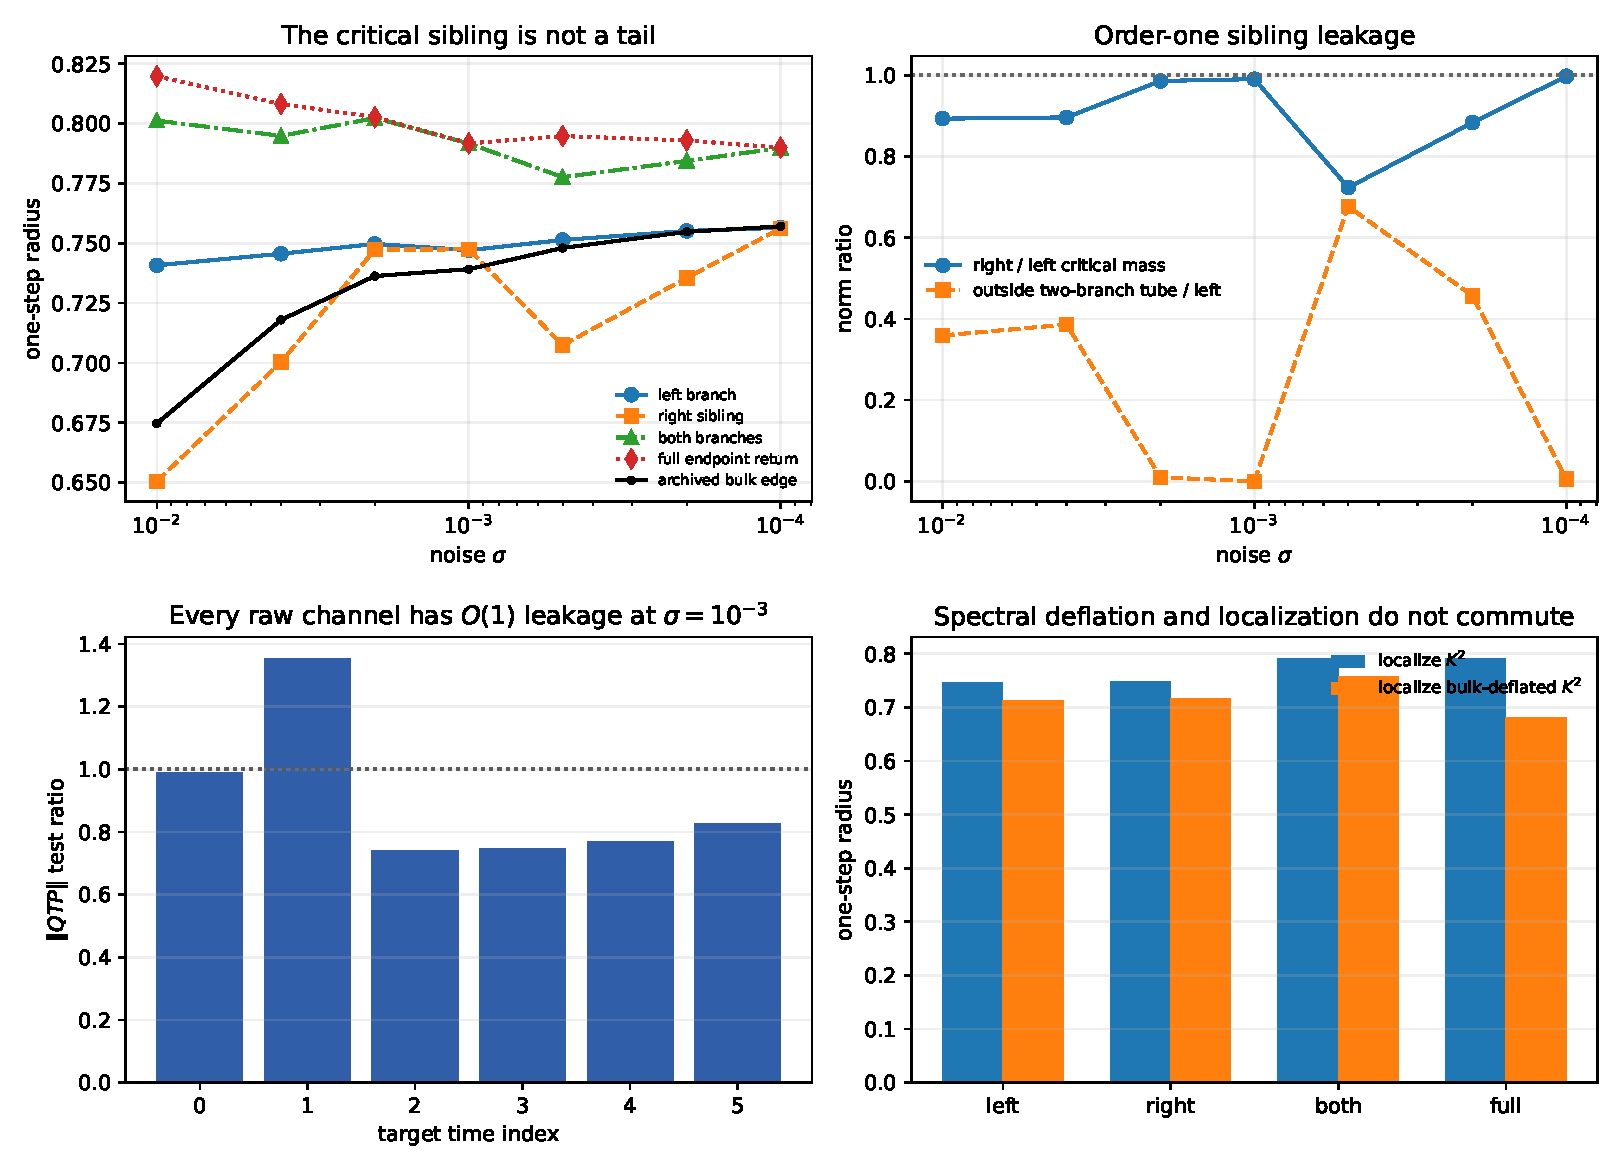
\includegraphics[width=\textwidth]{figures/critical_sibling_complement.pdf}
\caption{Complement-coupling audit.  Top left: one-branch, two-branch, and
unrestricted endpoint radii versus the archived physical bulk edge.  Top
right: sibling and fixed-window far exit masses relative to the retained
branch.  Bottom left: complement/local test ratios for all six component
channels at $\sigma=10^{-3}$.  Bottom right: local returns formed before and
after global Perron/parity deflation.  The comparisons are floating-point
diagnostics, not norm enclosures.}
\label{fig:complement-audit}
\end{figure}

The branch-complete positive return lies near $0.79$, above both the physical
bulk edge and the limiting pole radius $\lambda^{-1/2}=0.7718445\ldots$.
Therefore the successful left-branch radius cannot be justified by saying
that all omitted positive paths are asymptotically negligible.  Some
sector-dependent cancellation or extraction must occur before the physical
bulk determinant is obtained.

\subsection{Deflation--localization benchmark}

At $\sigma=10^{-3}$, sparse right and left eigenvectors resolve
\begin{equation}\label{eq:peripheral-values}
 \lambda_0=1.0000000000000002,
 \qquad
 \lambda_-=-0.996389276627418,
\end{equation}
with all four left/right residuals below $2.1\times10^{-15}$.  Applying the
rank-two deflated operator before every localization gives the following.

\begin{table}[H]
\centering
\small
\caption{Noncommutation of global Perron/parity deflation and packet
localization at $\sigma=10^{-3}$, $k=6$.}
\label{tab:deflation}
\begin{tabular}{lrr}
\toprule
return & localize $\cK_\sigma^2$ & localize $K_{\rm b}^2$\\
\midrule
left  &0.747069&0.712178\\
right &0.747420&0.716453\\
both  &0.791673&0.756816\\
full endpoint&0.791700&0.681532\\
\bottomrule
\end{tabular}
\end{table}

The shifts are far larger than the $1/k$-scale radial precision sought from
a perturbative cloud theorem.  This one-noise benchmark is not an asymptotic
claim; it demonstrates that the rank-two terms in
\eqref{eq:localized-deflation} cannot simply be omitted from the proposed
effective block.

\subsection{Floquet and Schur algebra audit}

A random real $3\times3$ operator at period five verifies the exact finite
identities independently.  The maximum eigenvalue matching error in
\eqref{eq:fourier-decomposition} is $1.50\times10^{-15}$, the maximum relative
determinant error in \eqref{eq:lift-determinant} is
$1.11\times10^{-16}$, and the maximum Schur factorization error in
\eqref{eq:feshbach-determinant} is $3.49\times10^{-17}$.  For the deliberately
non-invariant phase-dependent test projection, the self-energy/local norm
ratio ranges from $1.57$ to $4.30$ at three nonsingular spectral parameters.
These last random-matrix ratios are only a software test of a non-small
regime, not evidence about the Gaussian asymptotic.

At $\sigma=10^{-2}$, the leading physical Nystr\"om eigenvalues are squared
and rotated through the three component-time sectors.  The right panel of
\cref{fig:floquet-audit} shows the exact replication.  Each three-point ring
comes from one point in the left panel.

\begin{figure}[H]
\centering
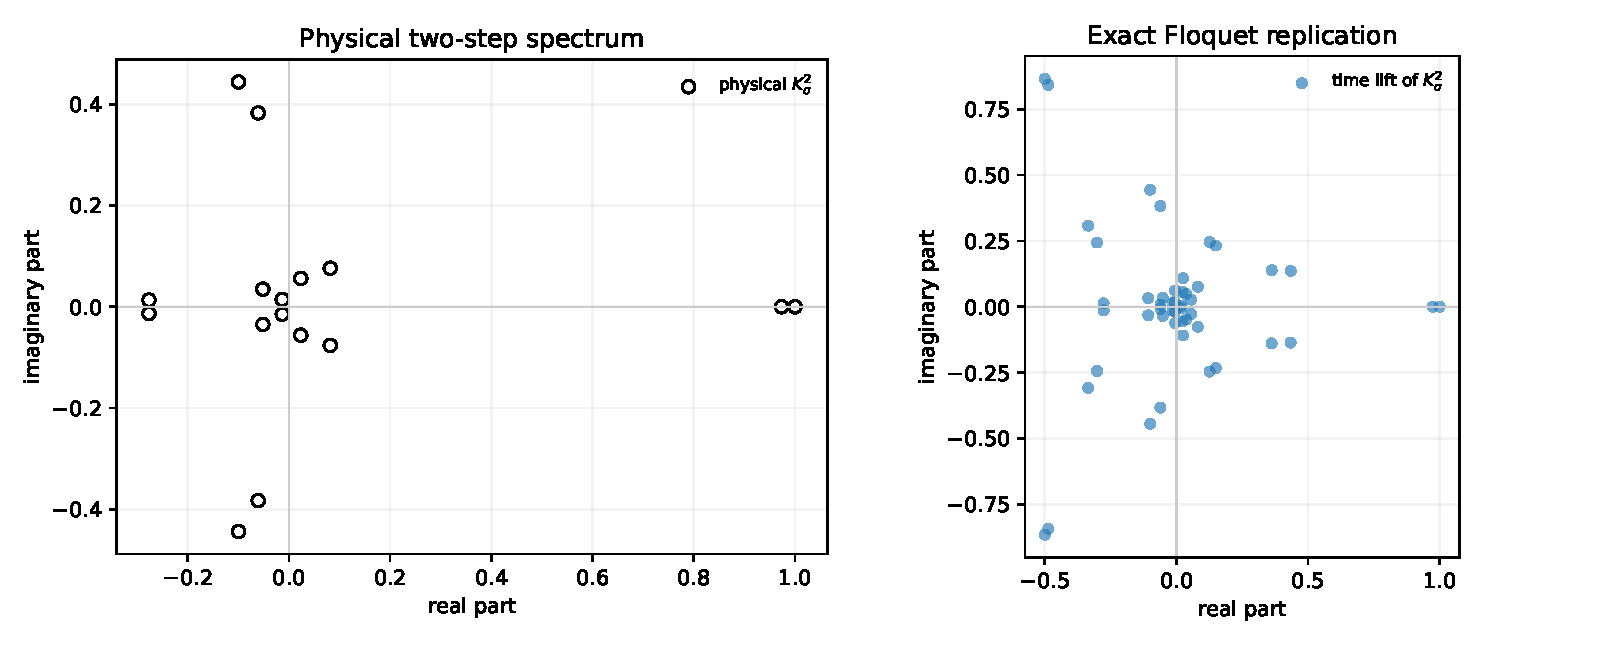
\includegraphics[width=0.96\textwidth]{figures/floquet_replication_no_go.pdf}
\caption{The physical two-step spectrum (left) and its exact time-unfolded
Floquet replication at component period three (right).  The extra rotated
points are eigenvalues of the time lift, not additional physical Markov
resonances.}
\label{fig:floquet-audit}
\end{figure}

\subsection{Reproducibility and numerical status}

The implementation tests the Fourier block decomposition, determinant
identity, phase projections, exact Schur factorization, branch-sum identity,
matrix-free endpoint returns, and rank-two deflation action.  The full audit
records all return values, residuals, leakage ratios, software versions,
source hashes, peripheral residuals, Floquet copies, and figures.  NumPy,
SciPy, and Matplotlib provide the numerical implementation
\citep{HarrisEtAl2020,VirtanenEtAl2020,Hunter2007}.  No calculation uses
interval arithmetic or supplies a non-normal pseudospectral enclosure.

\section{The corrected operator target}
\label{sec:corrected-route}

The failed strategy was specific:
\begin{equation}\label{eq:failed-strategy}
 \text{one branch}
 +\text{slowly growing windows}
 +\text{sector-free time lift}
 \quad\Longrightarrow?\quad
 \text{physical cloud block}.
\end{equation}
The critical-sibling theorem disproves small branch complement coupling, and
the Floquet theorem disproves the final counting inference.  A corrected
construction must change all three ingredients.

\begin{enumerate}[label=\textbf{R\arabic*.},leftmargin=3.1em]
 \item \textbf{Two-branch critical entrance.}
 Replace the scalar final packet by the vector
 $(\Gamma^-_{d,t},\Gamma^+_{d,t})$.  The corresponding return object is at
 least $2\times2$ in branch space.  Its symmetric and antisymmetric channels
 must be computed rather than selecting the left branch by hand.

 \item \textbf{Peripheral extraction inside the Grushin data.}
 Choose entrance and exit maps biorthogonal to $E_0$ and $E_-$ before
 localization.  Identity \eqref{eq:localized-deflation} then becomes part of
 the model, not a posteriori error.

 \item \textbf{Spectral-parameter closing phase.}
 Introduce a Floquet multiplier tied to the physical spectral parameter.
 The effective Hamiltonian should be a function $E_{-+}(\mu)$ whose closing
 condition selects a physical sector, rather than the spectrum of a fixed
 sector-free cyclic matrix.

 \item \textbf{Only then control the complement resolvent.}
 Decompose the remaining complement into far Gaussian tails and genuine bulk
 excursions.  The former may admit growing-window estimates; the latter
 require a resolvent bound after the branch and peripheral channels have been
 removed.
\end{enumerate}

A useful next theorem would derive the $2\times2$ critical return matrix and
identify which branch combination carries the parity-extracted determinant.
If one combination reproduces the RH-18 radius while the other is absorbed
by peripheral extraction, the program can return to a sector-resolved Schur
self-energy estimate.  If not, the single-cycle spectral interpretation must
be abandoned in favor of the already rigorous trace/determinant route.

\section{Discussion}
\label{sec:discussion}

\subsection{What the negative result changes}

The RH-18 branch block remains a well-defined positive compact operator, and
its principal radius remains an accurate numerical predictor of the outer
bulk edge.  What changes is the proposed proof mechanism.  The omitted right
branch has equal asymptotic critical mass and an almost equal finite return;
therefore the left block is not isolated by Gaussian decay.  Moreover, its
exact root phases arise in a time-labeled space where such phases are present
for every physical eigenvalue by Fourier replication.

Thus two visually successful facts---the left radial match and the exact
local root ring---do not yet combine into a physical spectral theorem.  This
is precisely the kind of distinction a Feshbach analysis was meant to test.
The result prevents a plausible but invalid proof from being built on top of
the earlier numerical evidence.

\subsection{What remains intact}

The deterministic pole factor \eqref{eq:pole-factor} is a trace/determinant
theorem and is unaffected.  The half-logarithmic endpoint rank is a
singular-value theorem and is unaffected.  The boundary-cycle multiplier,
Riccati packet, conditioned critical profile, and local block root algebra
are also unchanged.  The archived full Markov cloud consists of genuinely
distinct computed eigenvalues; the Floquet theorem does not make those data
artificial.  It only shows that the time lift cannot certify their
distinctness.

The numerical near-equality
$R^{\rm full}\approx R^-+R^+$ at the smallest noise is informative.  It
suggests that the first correction should be a finite branch matrix rather
than an uncontrolled infinite complement.  This is a narrower and more
testable target than the original scalar Feshbach claim.

\subsection{No arithmetic or self-adjoint implication}

All operators here arise from one noisy quadratic map.  The roots of unity
in the time lift are a finite Floquet replication, not zeta zeros.  No result
constructs a self-adjoint Hilbert--P\'olya operator, proves a prime-power
trace formula, or implies the Riemann hypothesis.  The no-go theorem is an
operator-theoretic clarification internal to this dynamical model.

\section{Conclusion}

The complement gate gives a clear negative answer to the naive strategy.
The critical sibling omitted by the branch-isolated return has the same
asymptotic pullback mass as the retained branch, so off-block coupling cannot
be reduced to a Gaussian tail.  Independently, the full cyclic time lift is
an exact direct sum of rotated physical two-step operators.  Its root rings
are Floquet copies and cannot certify physical resonance multiplicity.

The exact Feshbach map remains valid, but completing the scalar local block
in the sector-free lift would solve the wrong counting problem.  Global
Perron/parity deflation also changes localized channels by leading rank-two
terms.  At the smallest computed noise, the right return is $99.48\%$ of the
left return and the two-branch return accounts for $99.81\%$ of the
unrestricted positive endpoint return, making the obstruction numerically
visible as well as analytic.

The route is narrowed rather than closed.  The next admissible object is a
two-branch, peripherally extracted, Floquet-sector effective Hamiltonian.  Its
symmetric and antisymmetric branch channels must be resolved before any
claim of small Schur self-energy or physical cloud multiplicity is made.
This is the precise operator problem left by the present boundary test.

\section*{Data and code availability}

The source code, tests, complete CSV and JSON audits, peripheral projectors,
Floquet replication data, figures, and manuscript are available with this
paper \citep{WangComplementCode2026}.

\bibliographystyle{plainnat}
\bibliography{references}

\end{document}
